\documentclass{article}
\usepackage{inputenc}
\usepackage{setspace}
\usepackage[margin=0.75in]{geometry}
\usepackage[style=numeric]{biblatex}
\addbibresource{../bibs/ref.bib}
\usepackage{float}
\usepackage{graphicx}
\graphicspath{ {./images/} }


\onehalfspace
\setlength{\parindent}{0pt}
\setlength{\parskip}{1em}



\begin{document}

\begin{center}
  \LARGE{\textbf{Real-world Functional Programming}} \\
  \Large{Coursework Part II Report} \\
  \normalsize{14274056 Junsong Yang (psyjy3)} \\
  \today
\end{center}


\begin{normalsize}
  \section{Task II.1}

  \begin{figure}[H]

    \begin{minipage}[b]{0.48\linewidth}
      \centering
      \centerline{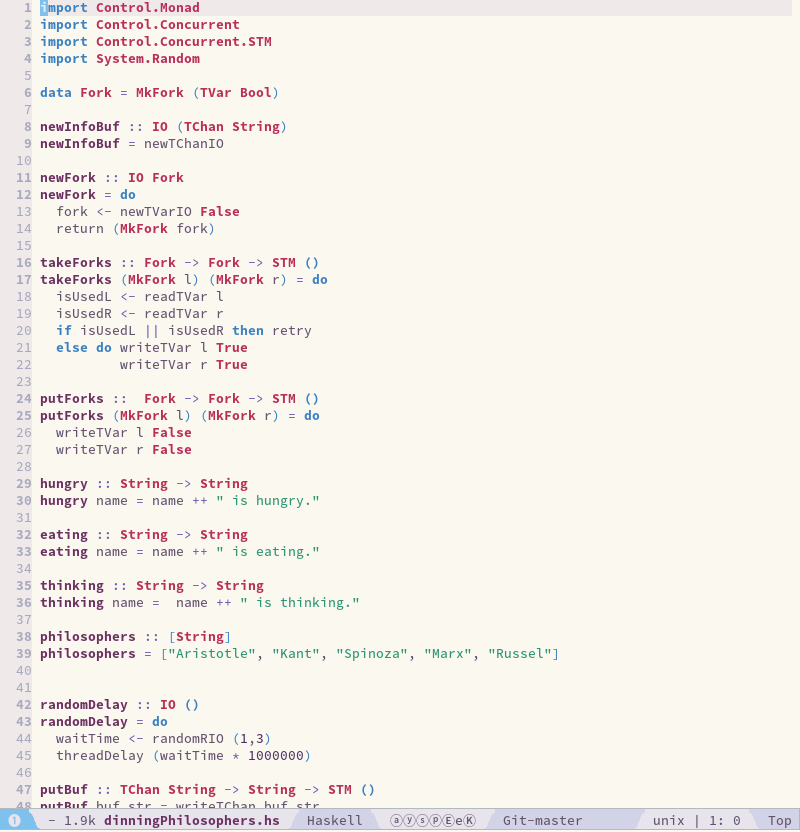
\includegraphics[width=8.5cm]{dinning1}}
      \centerline{ (a) Dinning Phhilosopher Part I}\medskip
    \end{minipage}
    \hfill
    \begin{minipage}[b]{0.48\linewidth}
      \centering
      \centerline{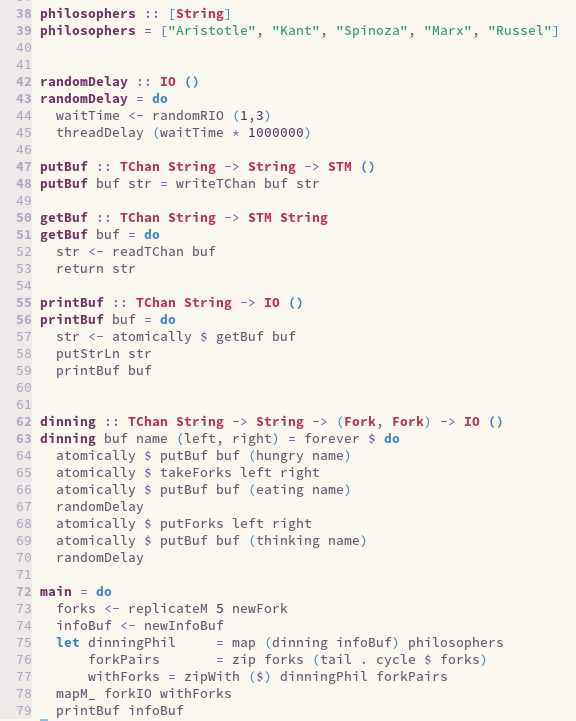
\includegraphics[width=8.5cm, height=12.5cm]{dinning2}}
      \centerline{ (b) Dinning Phhilosopher Part II }\medskip
    \end{minipage}
    \caption{Dinning Phhilosopher Part I}
    \label{fig:dinning}
  \end{figure}

  Figure \ref{fig:dinning} contains two figures that show the full
  implementation of dinning philosopher using STM. Starting with figure
  \ref{fig:dinning} (a), the Fork type is defined with a constructor called
  MkFork which take a TVar with a Bool as a input. If the boolean inside the
  TVar is false then this fork is available to be used otherwise this fork is
  already taken. The newInfoBuf function will return a TChan with String wrapped
  in IO monad to be used later to store logs that indicate the running state of
  each thread. The newFork function will return a Fork wrapped in IO monad with
  the boolean value set to false.

  The next two function takeForks and putForks are related to require and
  release resources. The takeForks function takes two Fork as input. This
  function will first check if the two Forks are both available. The two Forks
  can only be used if they are both available as the same time. Otherwise, this
  function will keep retrying untill both Forks can be required. The putForks
  function is simple just release the two Forks by setting the boolean to true.

  The next three functoins hungry, eating, thinking are just dummy functoin that
  concatenate the name of philosopher with corresponding information. These will
  later be put into the infoBuf(TChan String). The names of philosophers are
  defined as a list of string as figure \ref{fig:dinning} (b) shows.

  The randomDelay will call threadDelay to delay the running thread randomly
  from 1 to 3 seconds. The next three functions, putBuf, getBuf printBuf are
  operations related to the infoBuf(TChan String) that is used to store the logs
  for running thread. The putBuf function will just store string to the
  infoBuf(TChan String), the getBuf function will return the string stored in
  TChan and wrap in STM monad. The printBuf will just print the string stored in
  TChan.

  The dinning function is contains the implementation of dinning philosophers.
  This function takes a TChan String(used to store logs), a string(indicates
  philosopher's names), and a pair of Fork as input. This function will first
  store a log in the TChan that indicates the philosopher is hungry. Then, this
  function will trying to aquire the Fork using takeForks function. If the
  forks are aquired successfully, another log will be stored in the TChan that
  suggests the philosopher is eating. Followed by a random delay from 1 to 3
  seconds, the forks qill be released using putForks function and corresponding
  log will be put into the TChan. Finally, the function ended with another
  random delay.

  The main function will first initialise 5 Forks using newFork function and a
  infoBuf using newInfoBuf functions. Then the philosophers' name will be
  bundled with the dinning function using map. Then, a infinite list of pair of
  forks will be generated such that each fork in the pair is distinct from the
  other. Followed by coupling pairs of forks with the dinning function, a list
  of runnable functions is made. Finally, the main function will run those
  function by mapping forkIO function to the runnable dinning functions while
  the printBuf function is called to print the logs of those running thread.

   \begin{figure}[H]

    \begin{minipage}[b]{0.24\linewidth}
      \centering
      \centerline{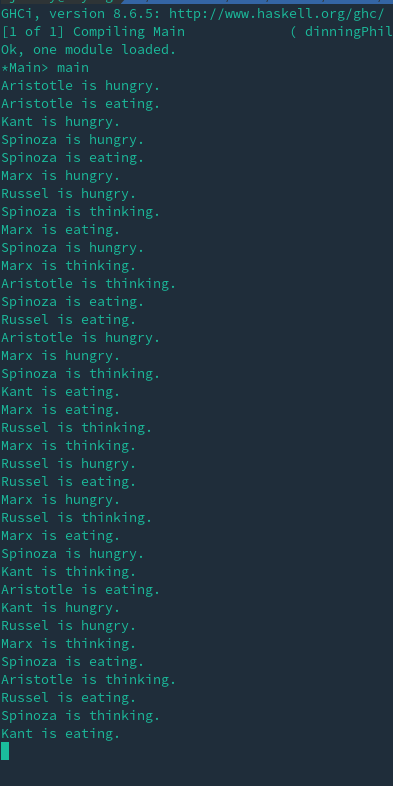
\includegraphics[width=4.0cm]{dinning10s}}
      \centerline{ (a) running at 10s}\medskip
    \end{minipage}
    \hfill
    \begin{minipage}[b]{0.24\linewidth}
      \centering
      \centerline{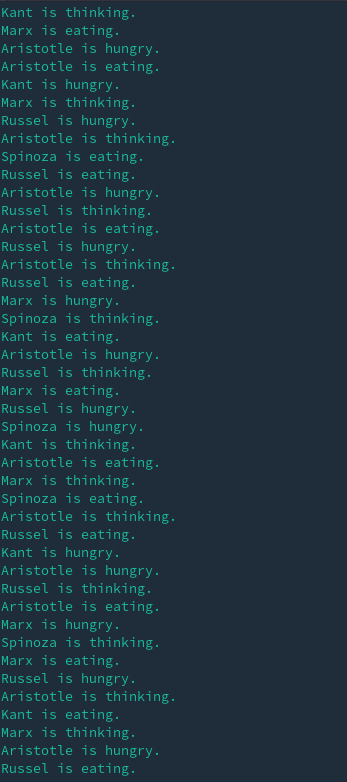
\includegraphics[width=4.0cm]{dinngin1m}}
      \centerline{ (b) running at 1m}\medskip
    \end{minipage}
    \hfill
    \begin{minipage}[b]{0.24\linewidth}
      \centering
      \centerline{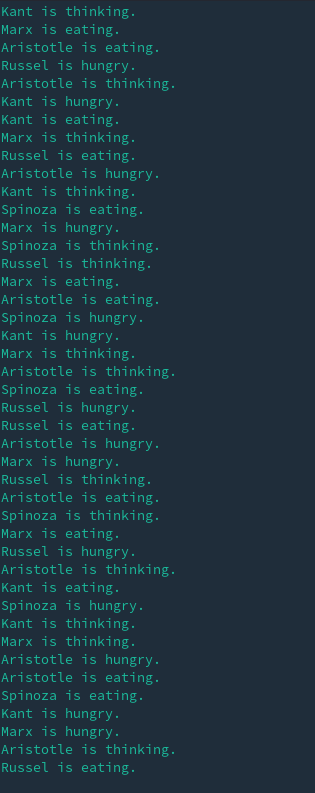
\includegraphics[width=4.0cm]{dinning2m}}
      \centerline{ (c) running at 2m}\medskip
    \end{minipage}
    \hfill
    \begin{minipage}[b]{0.24\linewidth}
      \centering
      \centerline{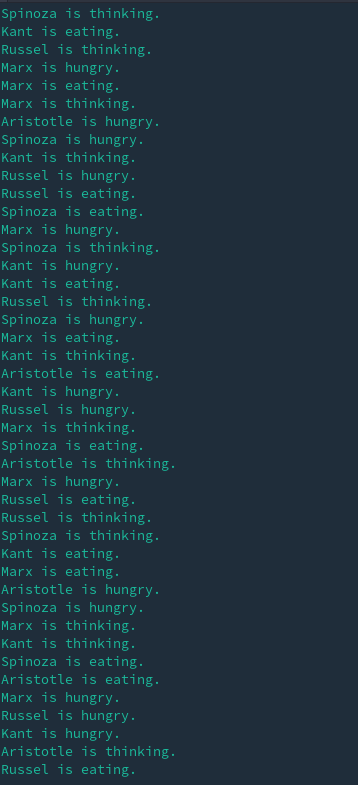
\includegraphics[width=4.0cm]{dinning4m}}
      \centerline{ (b) running at 4m}\medskip
    \end{minipage}

    \caption{Dinning Philosopher Running at Defferent Point of Time}
    \label{fig:drunning}
  \end{figure}

  Figure \ref{fig:drunning} contains four figures that shows this implementation
  running non-stop for four minutes. These sample output of the running program
  suggests that this implementation is working and without deadlocks.

  



  \section{Task II.2}
  
  \begin{figure}[H]
    \centering
    \centerline{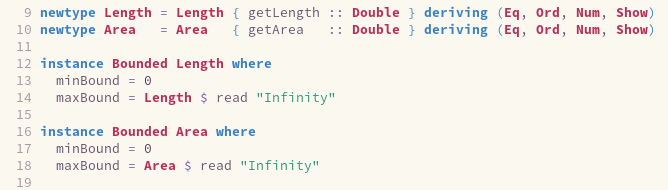
\includegraphics[scale=0.4]{StatsBonusBound}}
    \caption{newtype Bounded}
    \label{fig:bounded}
  \end{figure}

  
  \begin{figure}[H]

    \begin{minipage}[b]{0.48\linewidth}
      \centering
      \centerline{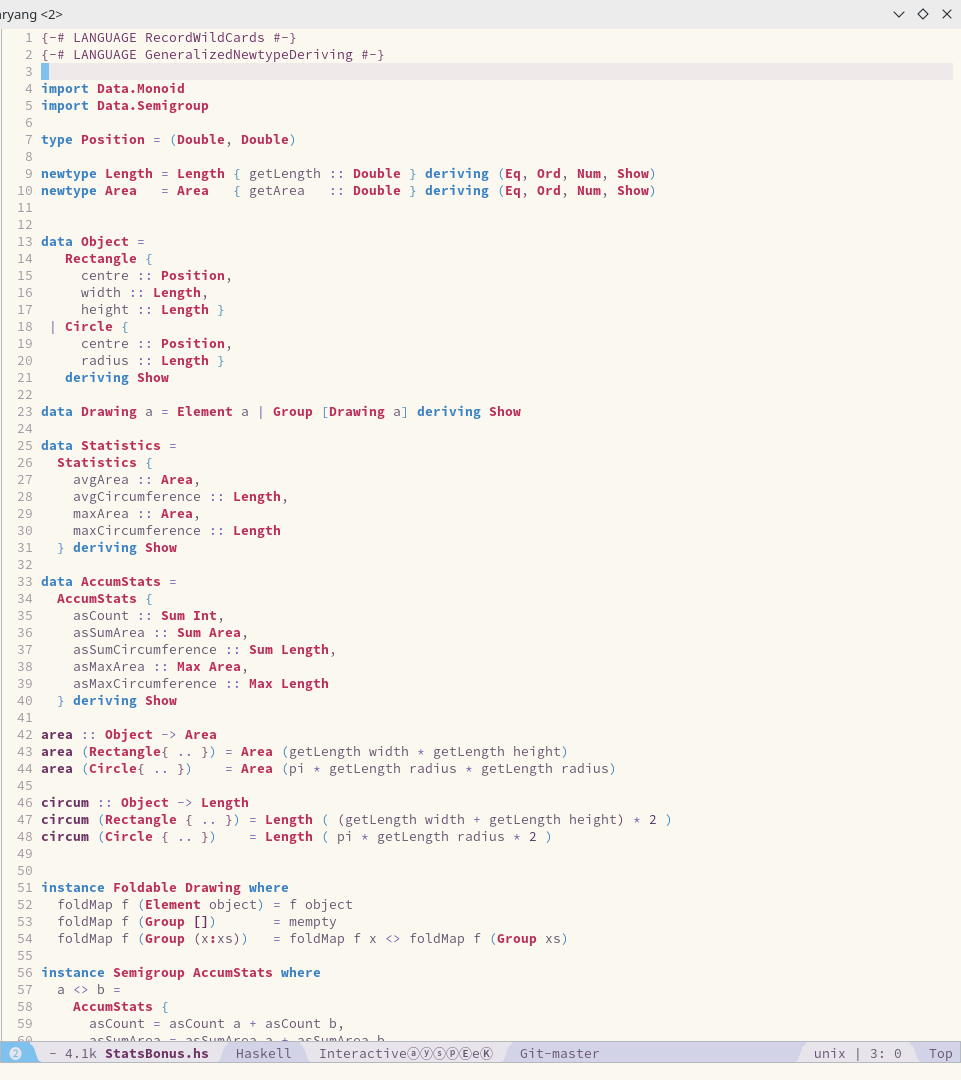
\includegraphics[width=8.0cm]{StatsBonus}}
      % \vspace{1.5cm}
      \centerline{ (a) Recursive Statistics for newtype}\medskip
    \end{minipage}
    \hfill
    \begin{minipage}[b]{0.48\linewidth}
      \centering
      \centerline{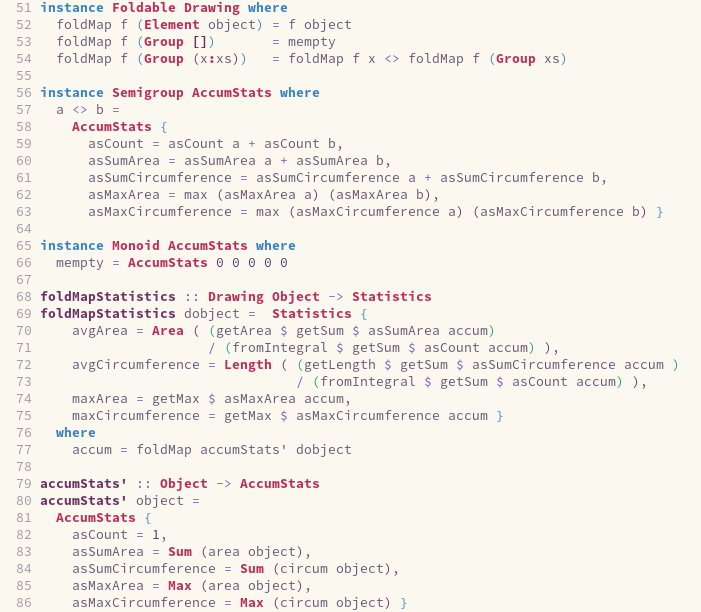
\includegraphics[width=8.0cm]{StatsBonusFoldMap}}
      % \vspace{1.5cm}
      \centerline{ (b) Statistics using foldMap for newtype}\medskip
    \end{minipage}
    % 
    \caption{TaskI.5 3}
    \label{fig:taskI.5.3}
    % 
  \end{figure}

  
\end{document}


